\documentclass[tikz,border=12pt]{standalone}
\usepackage{amsmath,amssymb}
\usetikzlibrary{arrows.meta,calc}

\begin{document}
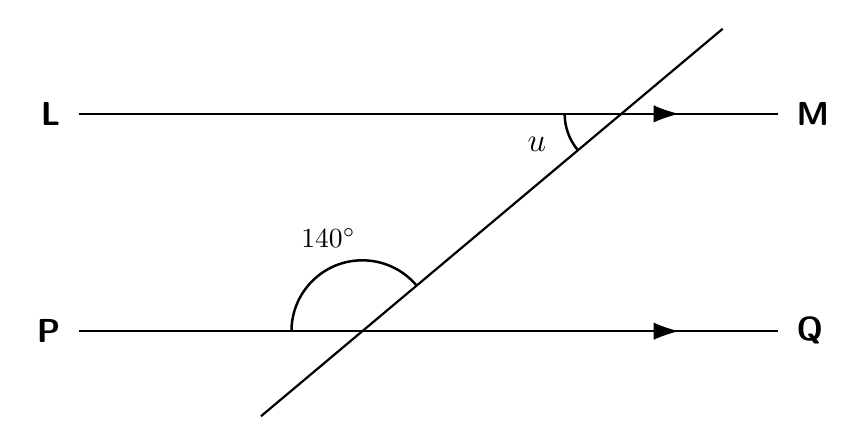
\begin{tikzpicture}[scale=1.2]
    % Transversal crossing parallel lines LM and PQ (adapted from diagram_02 template)
    % Transversal rises at 40 deg to the horizontal: acute angles = 40, obtuse = 140
    \pgfmathsetmacro{\ang}{40}
    \pgfmathsetmacro{\ytop}{2.3}
    \pgfmathsetmacro{\xtop}{\ytop / tan(\ang)}

    \coordinate (Ibot) at (0, 0);
    \coordinate (Itop) at (\xtop, \ytop);

    % Horizontal parallel lines
    \draw[thick] (-3.0, \ytop) node[left=3pt, font=\large\sffamily\bfseries] {L} -- (4.4, \ytop) node[right=3pt, font=\large\sffamily\bfseries] {M};
    \draw[thick] (-3.0, 0) node[left=3pt, font=\large\sffamily\bfseries] {P} -- (4.4, 0) node[right=3pt, font=\large\sffamily\bfseries] {Q};

    % Parallel indicator arrows
    \draw[-{Latex[length=3.2mm, width=2.2mm]}] (3.1, \ytop) -- (3.35, \ytop);
    \draw[-{Latex[length=3.2mm, width=2.2mm]}] (3.1, 0) -- (3.35, 0);

    % Transversal line extending symmetrically beyond both intersections
    \draw[thick] ($(Ibot) - ({1.4*cos(\ang)}, {1.4*sin(\ang)})$) -- ($(Itop) + ({1.4*cos(\ang)}, {1.4*sin(\ang)})$);

    % Given angle 140 deg at lower intersection: interior wedge between
    % ray 40 deg (toward upper intersection) and ray 180 deg (line to the left)
    \draw[line width=0.9pt] ($(Ibot) + (40:0.75)$) arc (40:180:0.75);
    \node[font=\bfseries] at ($(Ibot) + (110:1.05)$) {$140^\circ$};

    % Unknown u at upper intersection: interior wedge between ray 180 deg
    % (line to the left) and ray 220 deg (transversal toward lower intersection)
    \draw[line width=0.9pt] ($(Itop) + (180:0.6)$) arc (180:220:0.6);
    \node[font=\large\bfseries] at ($(Itop) + (200:0.95)$) {$u$};
\end{tikzpicture}
\end{document}
